\begin{frame}{PETSc Project Management}
  \begin{itemize}
  \item Public discussion at petsc-dev@mcs.anl.gov
    \begin{itemize}
    \item Private decisions disempower external contributors
    \item Remote team -- Matt, Lois, Jed, Karl, Mark
    \end{itemize}
  \item Git Workflow
  \item Barry is the ultimate arbiter, but grants a lot of leeway
  \item Developers have to care deeply about the project
  \item DOE Funding -- basic research only
    \begin{itemize}
    \item Does not fund ``support'', but PMs know we do it anyway
    \item Applied Math base program, SciDAC apps, other app partnerships
    \item Write Satish into grants, recognition with awards, authorship
    \end{itemize}
  \item Make development ``fun'' for external developers
    \begin{itemize}
    \item About 45 contributors in the past year
    \item 843/4195 commits from outside the ``core'' developers + Argonne staff
    \end{itemize}
  \end{itemize}
\end{frame}

\begin{frame}{Git Workflow Objectives}
  \begin{itemize}
  \item 'master' is always stable and ready to release
  \item features are complete and tested before appearing in 'master'
  \item commits are minimal logically coherent, reviewable, and testable units
  \item related commits go together so as to be reviewable and debuggable by specialist
  \item new development is not disrupted by others' features and bugs
  \item rapid collaboration between developers possible
  \item \texttt{git log -{}-first-parent maint..master} reads like a changelog
  \item bugs can be fixed once and anyone that needs the fix can obtain it without side-effects
  \end{itemize}
\end{frame}

\begin{frame}{Simplified gitworkflows(7)}
  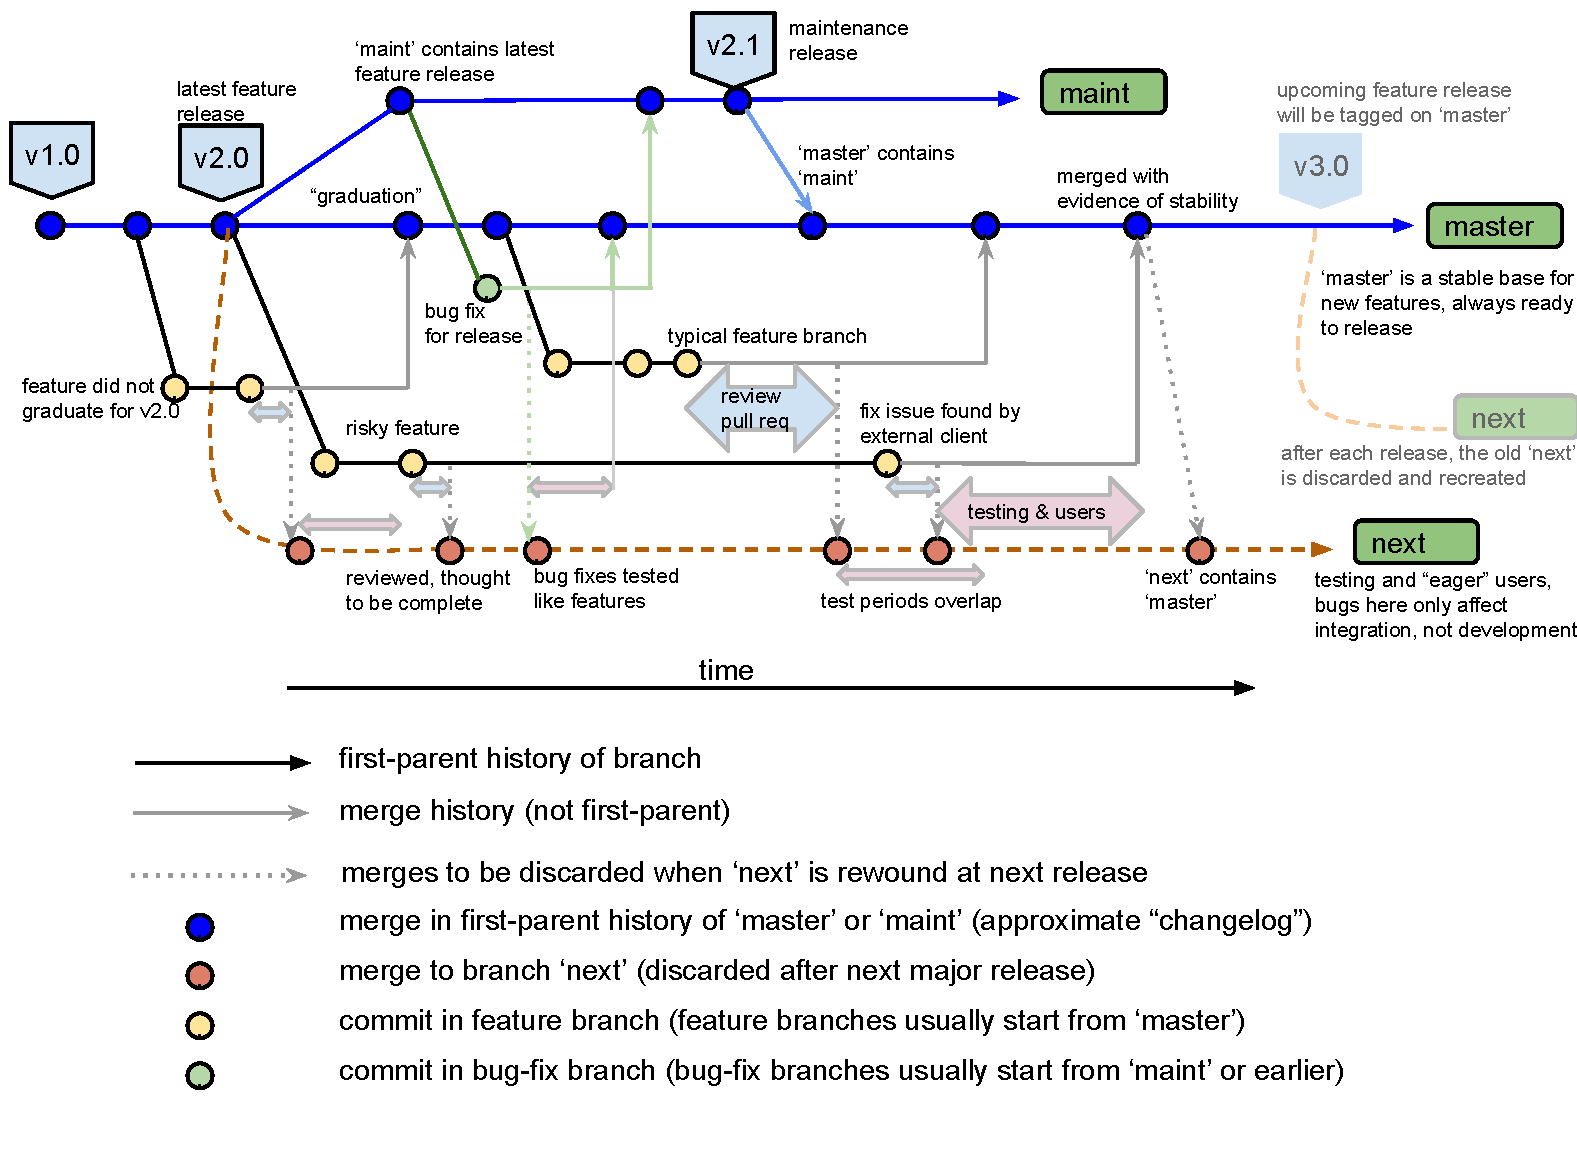
\includegraphics[width=\textwidth]{figures/Git/simplified-gitworkflows7.pdf}
\end{frame}
